\chapter{Introduction to electronics}

\section{Overview}

This lab will introduce you to a few basic electronic principles by trying them in action. You'll learn how to measure voltage, amperage, and resistance using a multimeter. Before you do this lab, you should familiarize yourself with the solderless breadboard and make yourself a power connector.
Click any image to see the larger version.


\section{Parts}

To do this, you'll need:

Solderless breadboard

\begin{figure}[!htb]
 \centering
 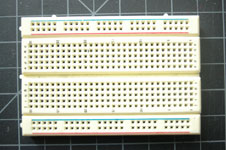
\includegraphics[scale=1.0]{img/electronics/breadboard.jpg}
 \caption{Solderless breadboard}
 \label{Solderless breadboard}
\end{figure}

22-AWG hookup wire

\begin{figure}[!htb]
 \centering
 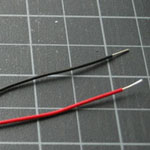
\includegraphics[scale=0.8]{img/electronics/hookup_wire.jpg}
 \caption{22-AWG hookup wire}
 \label{22-AWG hookup wire}
\end{figure}

Voltage regulator

\begin{figure}[!htb]
 \centering
 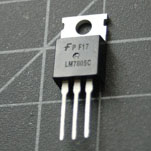
\includegraphics[scale=0.8]{img/electronics/voltage_reg.jpg}
 \caption{voltage regulator}
 \label{voltage regulator}
\end{figure}

Soldered DC Power Jack

\begin{figure}[!htb]
 \centering
 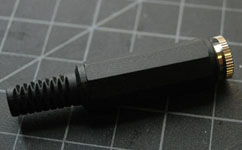
\includegraphics[scale=0.8]{img/electronics/power_connector.jpg}
 \caption{Soldered DC Power Jack}
 \label{Soldered DC Power Jack}
\end{figure}

Wire Strippers

\begin{figure}[!htb]
 \centering
 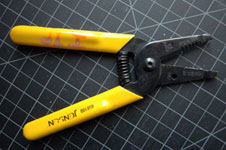
\includegraphics[scale=0.8]{img/electronics/wire_strippers.jpg}
 \caption{wire strippers}
 \label{wire strippers}
\end{figure}

Light Emiting Diodes, LED

\begin{figure}[!htb]
 \centering
 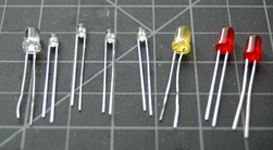
\includegraphics[scale=0.8]{img/electronics/leds.jpg}
 \caption{Light Emiting Diodes, LED}
 \label{Light Emiting Diodes, LED}
\end{figure}

10Kohm potentiometer

\begin{figure}[!htb]
 \centering
 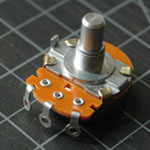
\includegraphics[scale=0.8]{img/electronics/potentiometer.jpg}
 \caption{10Kohm 10Kohm potentiometer}
 \label{10Kohm potentiometer}
\end{figure}

220-ohm resistors

\begin{figure}[!htb]
 \centering
 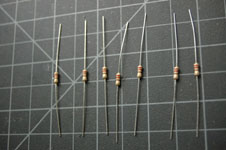
\includegraphics[scale=0.8]{img/electronics/resistors.jpg}
 \caption{220-ohm resistors}
 \label{220-ohm resistors}
\end{figure}

switch

\begin{figure}[!htb]
 \centering
 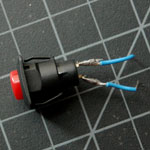
\includegraphics[scale=0.8]{img/electronics/switch.jpg}
 \caption{switch}
 \label{switch}
\end{figure}

Multimeter

\begin{figure}[!htb]
 \centering
 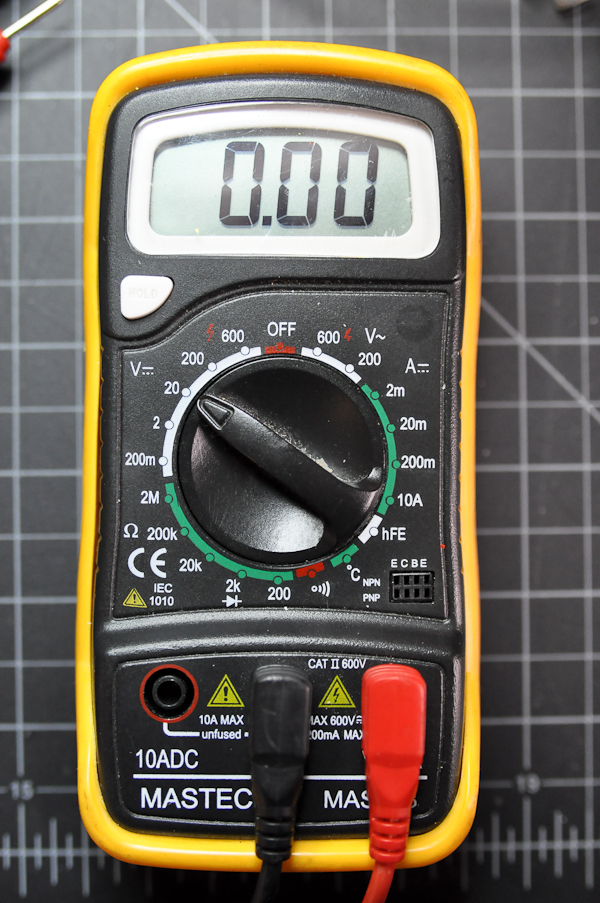
\includegraphics[scale=0.3]{img/electronics/multimeter_voltage.jpg}
 \caption{Multimeter}
 \label{Multimeter}
\end{figure}

\section{Measuring Continuity}


\begin{figure}[!htb]
 \centering
 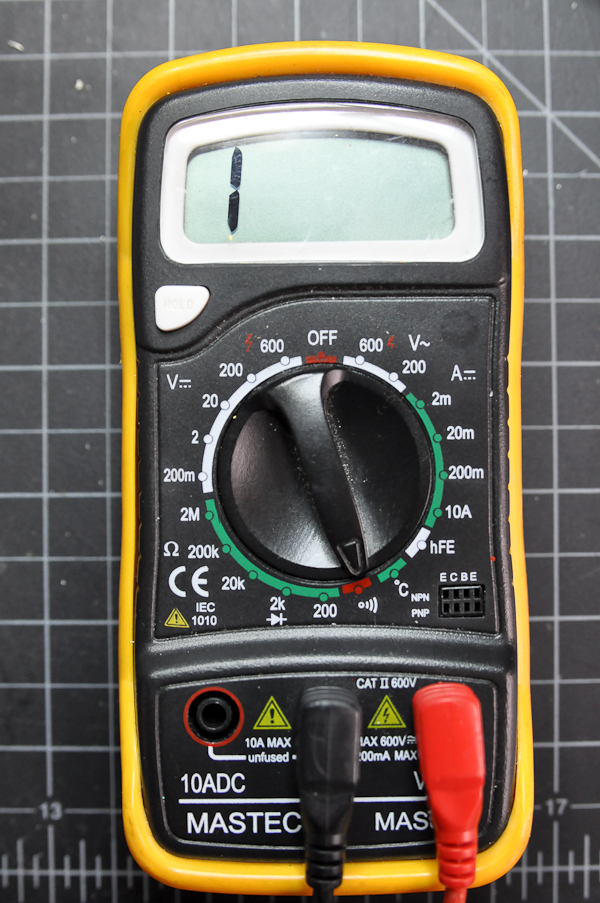
\includegraphics[scale=0.3]{img/electronics/multimeter_continuity.jpg}
 \caption{Multimeter set to measure continuity}
 \label{Multimeter set to measure continuity}
\end{figure}

Continuity is simply whether or not there is a connection between two points. You can use it to find with connections on a switch or pushbutton are connected when you press the button. You can also use it to measure whether there's a break in a wire, or whether a given material conducts electricity. Set your meter as shown here, and try touching the leads together. The meter should beep.
Now try touching the leads to two ends of a wire. Again, the meter should beep. The wire conducts electricity. There is a continuous flow of electricity from one end of the wire to another.
Now try touching two points on a switch. Do you get a beep? What happens when you switch the switch? Beep or no beep?
Put a wire in one hole of a breadboard. Then put another wire in another hole, chosen at random. Measure continuity between the two wires. Did you get what you expected?
Try measuring the continuity across your hand. Do you get anything? Why or why not? You probably don't because the resistance across your skin is so high that it doesn't register as a continuous conductor. It can conduct small amounts of current though. You don't want your body to carry high amounts of current or voltage though, because it can damage or kill you.

\section{Resistance of a component}

Resistance is a material property of a component, like a resistor or a wire. To measure the resistance of a component, you have to remove the component from the circuit. To measure resistance, turn your meter to the setting marked with the Greek letter Omega %(Ω):

\begin{figure}[!htb]
 \centering
 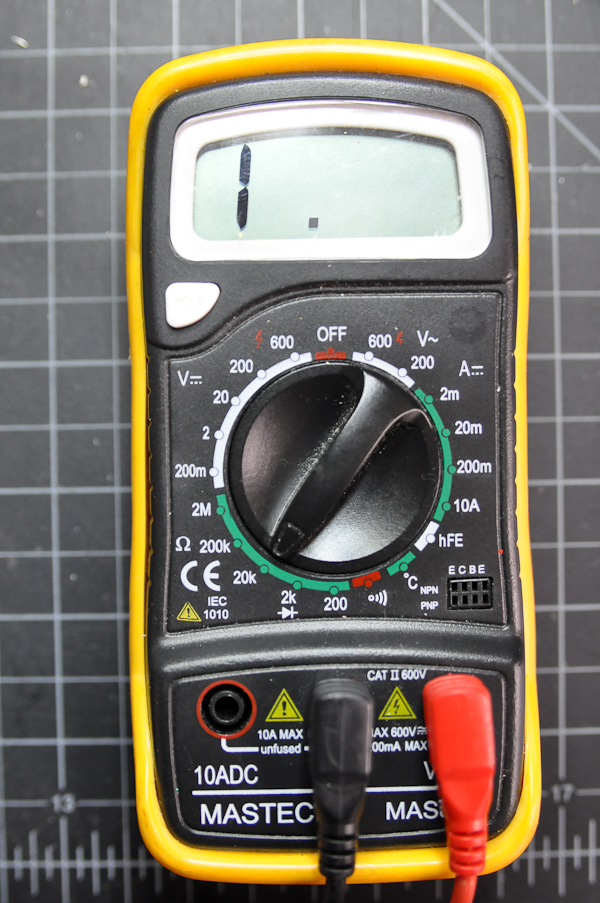
\includegraphics[scale=0.3]{img/electronics/multimeter_resistance.jpg}
 \caption{multimeter set to measure resistance}
 \label{multimeter set to measure resistance}
\end{figure}

Ideally, you want the meter set to the approximate range, and slightly higher than, of the component's resistance. For example, to measure a 10Kilohm resistance, you'd choose 20K, because 10K and 20K are in the same order of magnitude. For a 50K resistance, you'd have to step up to 200K, and so forth. If you don't know the component's resistance, start with the meter set to a high reading, like 2M (2 Megaohms). If you get a reading of zero, turn the meter one step lower, and keep doing so until you get a good reading.

\begin{figure}[!htb]
 \centering
 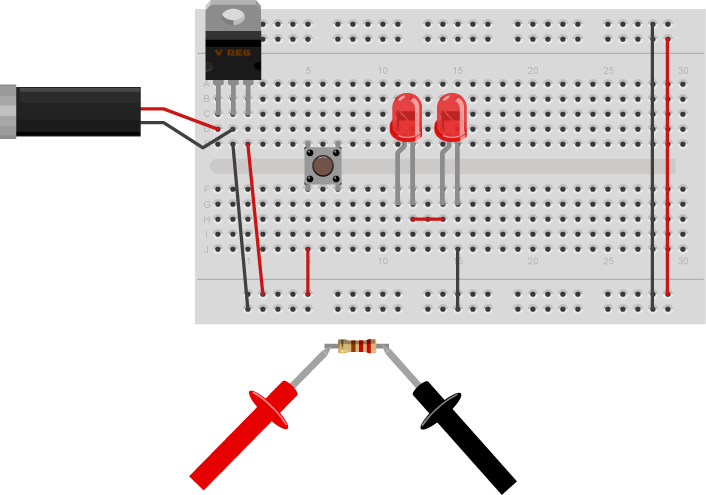
\includegraphics[scale=0.8]{img/electronics/measuring_resistance.jpg}
 \caption{measuring resistance. Note that this circuit is not complete.}
 \label{measuring resistance. Note that this circuit is not complete.}
\end{figure}

Not all components will register resistance. For example, a wire will ideally register 0 ohms, because you want wires to have as little resistance as possible so they don't affect the circuit. The longer the wire, the greater the resistance, however. Likewise, switches have ideally zero resistance.

The circuit shown is not complete. The resistor connecting the LED to ground has been removed to measure its resistance. To measure resistance of a component, you must remove it from the circuit.

If you measure the resistance of a diode, you may see a number flash briefly on the meter, then disappear. This is because diodes ideally have little or no resistance once voltage is flowing through them, but have what's called a forward bias, a minimum voltage needed to get current flowing. Before you reach the forward bias voltage, the diode's resistance is ideally infinite. After you reach it, the resistance is ideally zero. There are no ideals in electronics, however, which is why you saw a voltage drop across the diodes in the circuits above.

Try measuring the reistance across your hand. Set the meter really high, perhaps 2Megaohms Do you get anything? Why or why not? Make your palm sweaty and try again. What happened?

\section{Measuring Voltage}

The first thing you should do when working with electronic circuits is to get comfortable checking voltages in the circuit. Wire a 7805 5-volt voltage regulator on a breadboard as shown in the breadboard lab and connect it to power.The NYU Computer store, Radio Shack, and just about every electronics store will carry the voltage regulator, but if you don't have one, you can use the 5V output from an Arduino as well.

\begin{figure}[!htb]
 \centering
 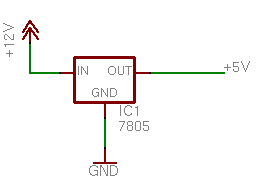
\includegraphics[scale=0.8]{img/electronics/5v_reg_sch.png}
 \caption{5v reg sch}
 \label{5v reg sch}
\end{figure}

\begin{figure}[!htb]
 \centering
 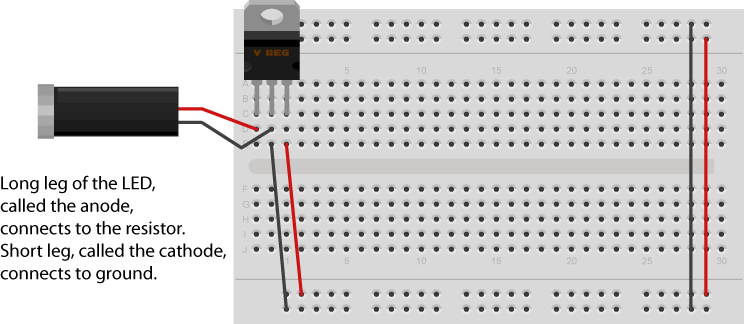
\includegraphics[scale=0.8]{img/electronics/breadboard_5V_reg.png}
 \caption{breadboard 5V reg}
 \label{breadboard 5V reg}
\end{figure}

Now add an LED and a 220-ohm resistor to the breadboard like so:

\begin{figure}[!htb]
 \centering
 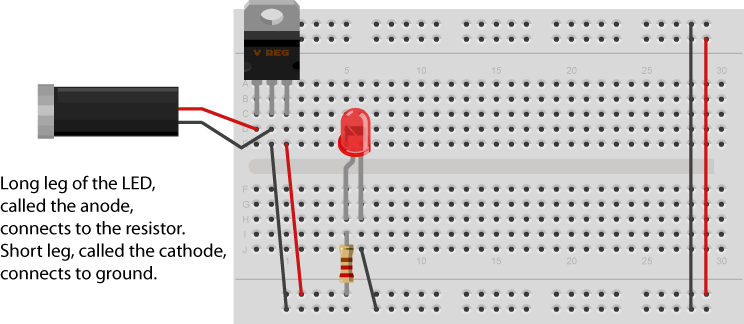
\includegraphics[scale=0.8]{img/electronics/breadboard_LED.png}
 \caption{breadboard LED}
 \label{breadboard LED}
\end{figure}

\begin{figure}[!htb]
 \centering
 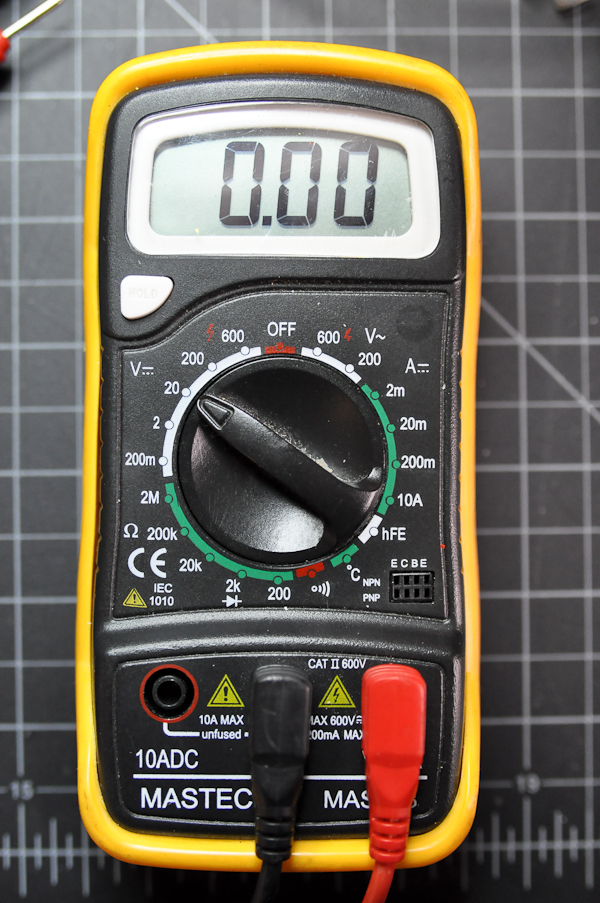
\includegraphics[scale=0.3]{img/electronics/multimeter_voltage.jpg}
 \caption{Multimeter set to measure DC voltage}
 \label{Multimeter set to measure DC voltage}
\end{figure}

Correct meter probe placement for measuring the voltage of an LED
made with Fritzing

Voltage is a measure of the difference in electrical energy between two points in a circuit. It's always measured between two points in a circuit. Measuring the voltage between the two sides of a component like an LED tells you how much voltage that component uses. This is known as measuring the voltage "across" the component. When you're measuring voltage across a component, you're putting the meter in parallel with the component. In that case, the voltage across both should be the same.

\begin{figure}[!htb]
 \centering
 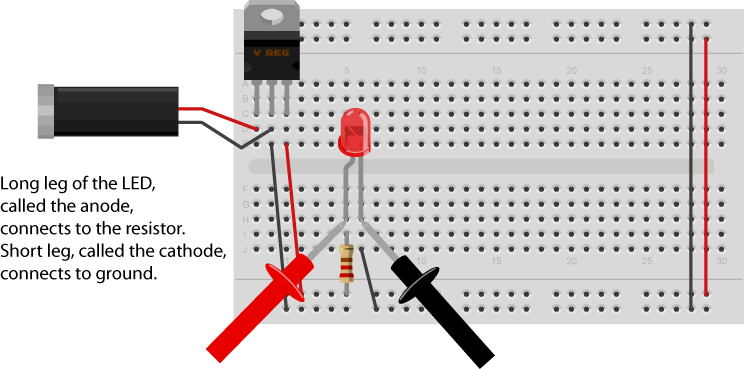
\includegraphics[scale=0.8]{img/electronics/breadboard_LED_meter.png}
 \caption{breadboard LED meter}
 \label{breadboard LED meter}
\end{figure}

Set your multimeter to measure DC volts. The voltage regulator you're using can take an input voltage range of about 8 to 15 volts, and it outputs 5 volts, so you know that no voltage you'll read in this circuit is over about 15 volts. If your meter has a variety of ranges for DC volts, choose a range that matches this. For example, many meters have a setting for 20 volts, meaning that they can read up to 20V DC at that setting. Measure for voltage between the power and ground bus rows on the breadboard. You should have 5 volts, or very close to that.

Did you get a negative voltage? That means you placed the red lead on the point of lower voltage, and the black lead on the point of higher voltage. In other words, you reversed the polarity.

\section{A Basic LED Circuit}

Now you're going to make your first working circuit. Disconnect the board from power and add an LED, a switch, and a resistor in series like so (remember, long leg (anode) goes to voltage, short leg (cathode) goes to ground):

\begin{figure}[!htb]
 \centering
 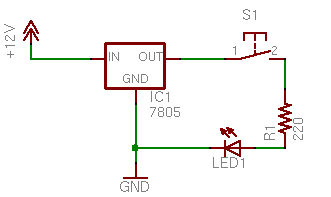
\includegraphics[scale=0.8]{img/electronics/led_switch_sch.png}
 \caption{led switch sch}
 \label{led switch sch}
\end{figure}

\begin{figure}[!htb]
 \centering
 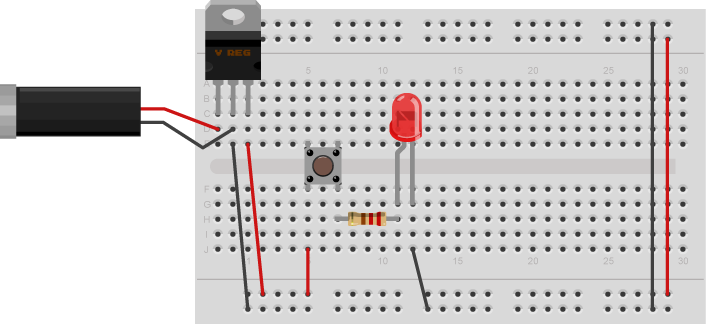
\includegraphics[scale=0.8]{img/electronics/breadboard_LED_switch.png}
 \caption{breadboard LED switch}
 \label{breadboard LED switch}
\end{figure}

Connect the board to your power supply and press the switch. It will illuminate the LED. Let go of the switch and it will turn the LED off again. By pressing the switch you are completing a circuit and allowing the resistor and LED to begin consuming electricity. The resistor is very important in this circuit as it protects the LED from being over-powered, which will eventually burn it out. A typical LED operates at a voltage of 2.0-2.6 volts (V) and consumes approximately 20 milliamps (mA). The resistor throttles the 5 volts coming from your voltage regulator and reduces the voltage to a level that is safer for the LED to consume. The higher the resistor value, the less electricity that will reach the LED. The lower the resistor value (with 0 ohms being no resistor at all), the more electricity that will reach the LED.

Now, while playing with the switch, measure the voltage across the switch as you did in the last step, both in the on position and the off position. Measure the voltage across the LED and the resistor as well. Does the total resistance across all the components add up to the voltage between power and ground on your board? Remember, in any circuit, all of the voltage must be used up. If the voltage across all the components doesn't add up, that indicates to you that some of the electrical energy is getting converted to light, heat, and other forms of energy. No component is 100% efficient, so there's always some loss.

\section{Components in Series}

Connect a pushbutton, a 220-ohm resistor and two LEDs in series from power to ground like so (remember, long leg of the LED (anode) goes to voltage, short leg (cathode) goes to ground):

\begin{figure}[!htb]
 \centering
 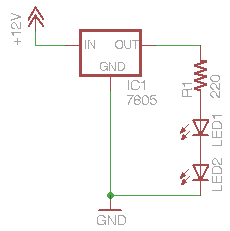
\includegraphics[scale=0.8]{img/electronics/leds_series_sch.png}
 \caption{leds series sch}
 \label{leds series sch}
\end{figure}

\begin{figure}[!htb]
 \centering
 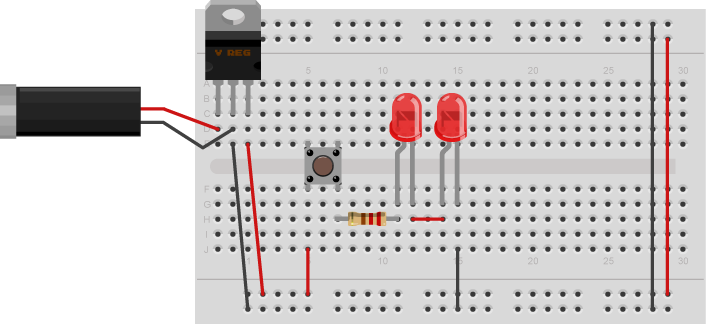
\includegraphics[scale=0.8]{img/electronics/leds_serial.png}
 \caption{leds serial}
 \label{leds serial}
\end{figure}

Measure the voltage across the resistor. Then measure the voltage across each LED. Does the total add up to the voltage from power to ground? If not, where does the missing voltage go?

\begin{figure}[!htb]
 \centering
 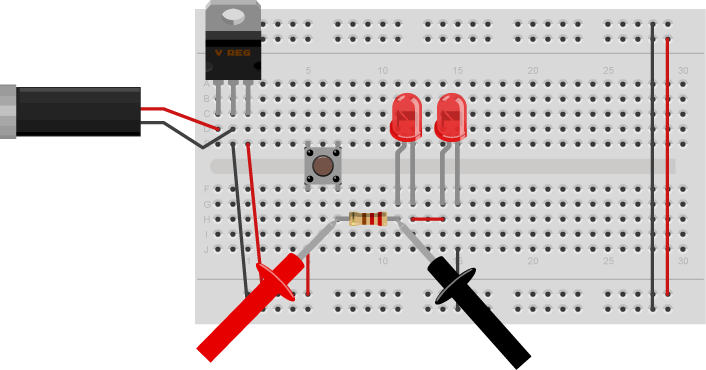
\includegraphics[scale=0.8]{img/electronics/voltage_across_resistor.png}
 \caption{measuring voltage across the resistor}
 \label{measuring voltage across the resistor}
\end{figure}

\begin{figure}[!htb]
 \centering
 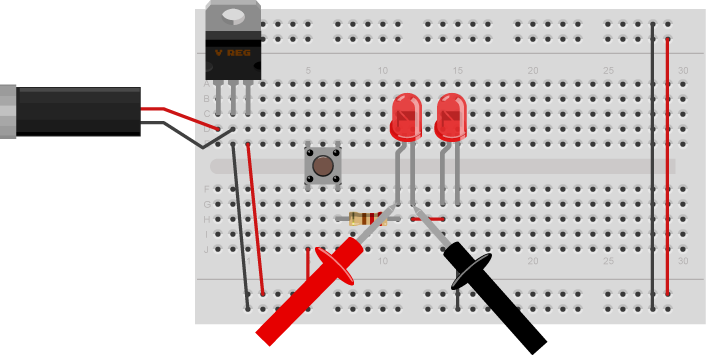
\includegraphics[scale=0.8]{img/electronics/voltage_across_led.png}
 \caption{measuring voltage across the resistor}
 \label{measuring voltage across the resistor}
\end{figure}

\begin{figure}[!htb]
 \centering
 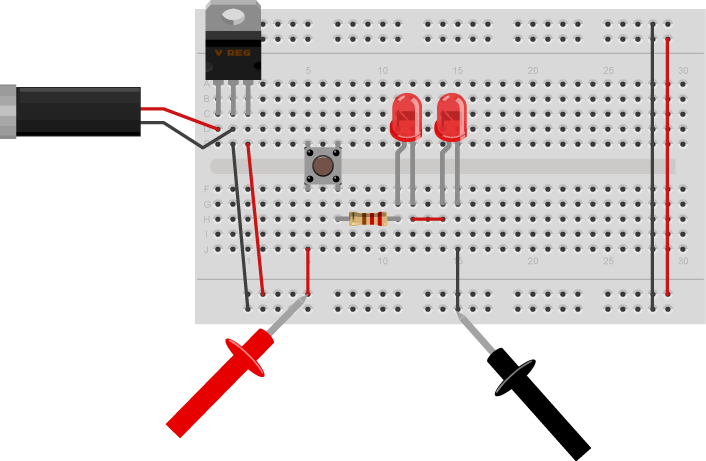
\includegraphics[scale=0.8]{img/electronics/voltage_power_ground.png}
 \caption{measuring voltage across the first LED}
 \label{measuring voltage across the first LED}
\end{figure}

measuring voltage across power and ground
Did you use two different color LEDs and get a different voltage drop across each one? That's normal. Because different color LEDs are made with different elements, and have slightly different voltage drops.
Did you get no reading when you measured? Did you remember to push the button before you took your reading?
Add a third LED in the series. Do they light? Why or why not?

\section{Components in parallel; measuring amperage}

Connect three LEDs in parallel like so (remember, long leg (anode) goes to voltage, short leg (cathode) goes to ground):

\begin{figure}[!htb]
 \centering
 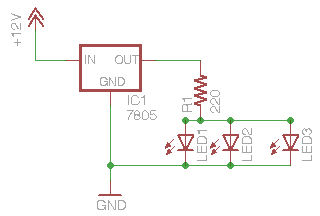
\includegraphics[scale=0.8]{img/electronics/leds_parallel_sch.png}
 \caption{leds parallel sch}
 \label{leds parallel sch}
\end{figure}

\begin{figure}[!htb]
 \centering
 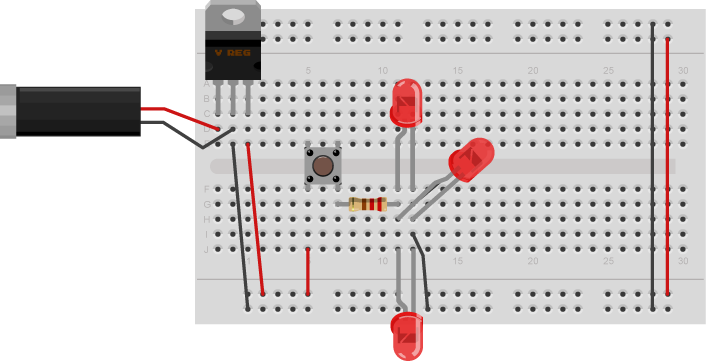
\includegraphics[scale=0.8]{img/electronics/leds_parallel.png}
 \caption{leds parallel}
 \label{leds parallel}
\end{figure}

Measure the voltage across each LED. It should be the same across each one.

\begin{figure}[!htb]
 \centering
 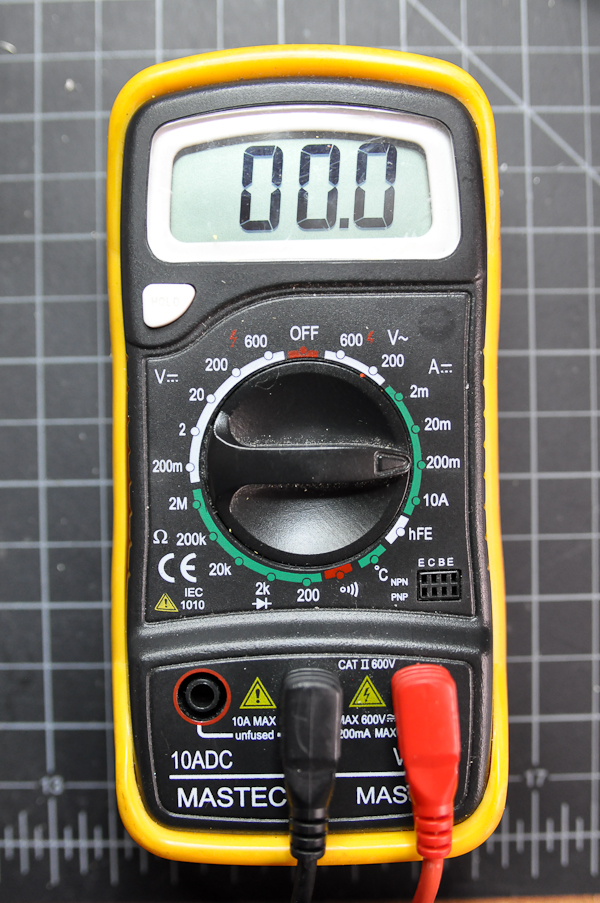
\includegraphics[scale=0.3]{img/electronics/multimeter_amperage_low.jpg}
 \caption{multimeter set to measure amperage up to 10A}
 \label{multimeter set to measure amperage up to 10A}
\end{figure}

Now you're going to read the amperage at various points in the circuit. Move your meter's red lead to the hole for measuring amperage. On many meters, there are three holes, one marked "Volts/Ohms/Hz", another marked "mA", and another marked "10A". The middle one can be used for measuring amperage when the expected amperage is less than 1A. The latter is for measuring high amperage, up to 10A. If you're not sure, it's best to use the hole for 10A. Then set your meter to measure DC amperage.

To measure the amperage through a given component, you need to place your meter in series with the component. When two components are in series, the amperage flowing through both of them is the same.

To measure the amperage through any one of the leds in this circuit, you'll need to disconnect one of its ends from the circuit (disconnect power first!) and use the meter to complete the circuit, like so:

\begin{figure}[!htb]
 \centering
 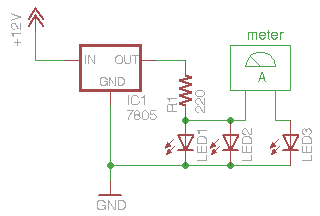
\includegraphics[scale=0.8]{img/electronics/metering_amps_sch.png}
 \caption{metering amps sch}
 \label{metering amps sch}
\end{figure}

\begin{figure}[!htb]
 \centering
 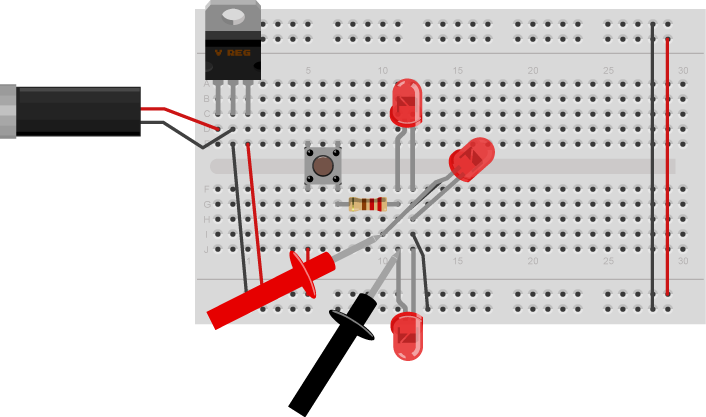
\includegraphics[scale=0.8]{img/electronics/breadboard_LED_parallel_meter.png}
 \caption{correct position for metering amperage.}
 \label{correct position for metering amperage.}
\end{figure}

Note that the second LED's anode leg has been moved, 
so there is no electrical connection with the other LED's anodes. 
The meter completes the circuit

You'll find that the amperage drawn by the LEDs is tiny, on the order of 10 or 20 milliamps at the most. That's normal for LEDs.
Make sure that you check which holes your leads are connected to when you're using a meter. Measuring amperage with the red lead in the voltage hole, or measuring voltage with it in the amperage holes is a good way to damage the meter.

\section{Generating a Variable Voltage with a Potentiometer}

\begin{figure}[!htb]
 \centering
 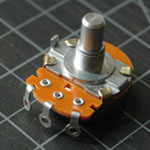
\includegraphics[scale=0.8]{img/electronics/potentiometer.jpg}
 \caption{10Kohm 10Kohm potentiometer}
 \label{10Kohm potentiometer}
\end{figure}

\begin{figure}[!htb]
 \centering
 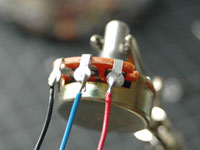
\includegraphics[scale=0.8]{img/electronics/pot_soldering.jpg}
 \caption{pot soldering}
 \label{pot soldering}
\end{figure}

In this last step, you'll generate a changing voltage using a potentiometer. A potentiometer is a resistor that can change its resistance. A potentiometer (or pot) has three connections. The outer leads are the ends of a fixed value resistor. The center lead connects to a wiper which slides along the fixed resistor. The resistance between the center lead and either of the outside leads changes as the pot's knob is moved.

\begin{figure}[!htb]
 \centering
 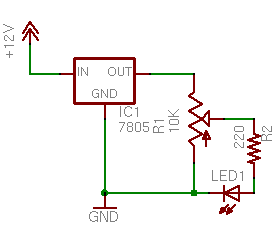
\includegraphics[scale=0.8]{img/electronics/led_pot_sch.png}
 \caption{led pot sch}
 \label{led pot sch}
\end{figure}

\begin{figure}[!htb]
 \centering
 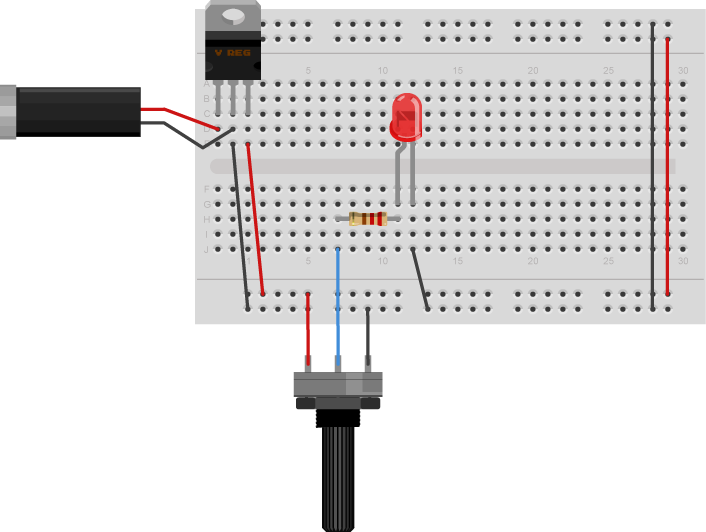
\includegraphics[scale=0.8]{img/electronics/breadboard_LED_pot.png}
 \caption{breadboard LED pot}
 \label{breadboard LED pot}
\end{figure}


Solder hook-up wires to the pot leads as shown here. Then connect the pot to an LED and a 220-ohm resistor using the following circuit:


As you turn the potentiometer from one end to the other, measure the voltage at the center position. The pot is acting as a voltage divider, dividing the 5V into two parts. As the voltage feeding the LED goes up or down, the LED gets brighter or dimmer. The 220-ohm resistor in the circuit protects the LED from overvoltage when the resistance between the pot's 5V lead and its center lead is 0 ohms.
Next, check out this lab.


